\section{Quantitative Comparison}
Here goes the quantitative comparison.

\subsection{Experiment Setup}
The experiment is setup with help of c...
The experiment is done  for 30 minutes with an interval of 30 seconds (without packet loss).

\textbf{Memory consumption}\\
Flyt den del til et afsnit med prototype implementation (før resultaterne)
How much memory usage...

\subsection{Bandwidth}
Measure number of bytes transferred between device and proxy.
More packet to send = more energy consumption

\textbf{First experiment:} Single transaction (non-coap,con-coap,coap over tcp).
\\ \\
	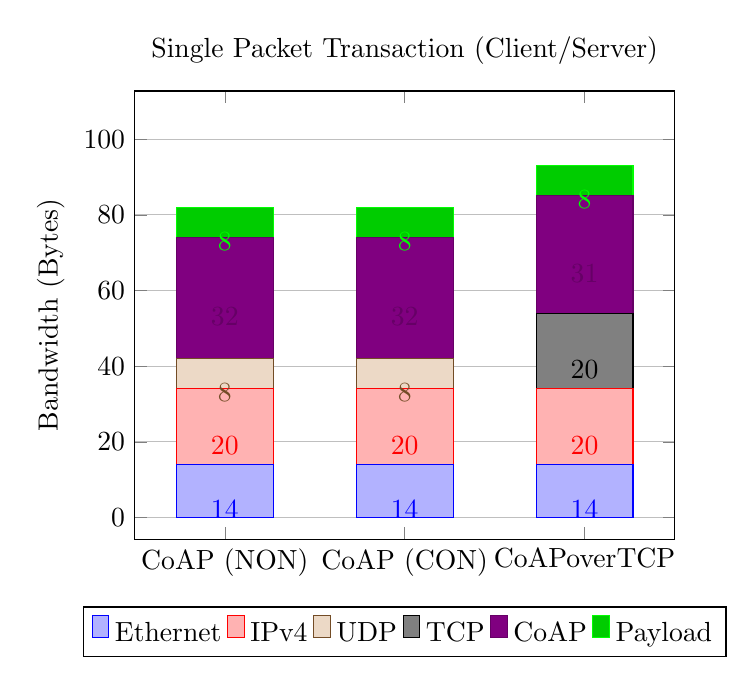
\begin{tikzpicture}
	\begin{axis}[
	 title={Single Packet Transaction (Client/Server)},
	ybar stacked,
	%ymax=50,
	ymajorgrids,
	bar width=35pt,
	%width=250pt,
	nodes near coords, 
	 %nodes near coords={\pgfmathprintnumber\pgfplotspointmeta \%},
	nodes near coords align={anchor=north},%Move values in bar
	every node near coord/.style={
	},
	enlargelimits=0.25,
	legend style={at={(0.5,-0.15)},
		anchor=north,legend columns=-1},
	%width=0.8*\textwidth,
	ylabel={Bandwidth (Bytes)},
	symbolic x coords={CoAP (NON), CoAP (CON), CoAPoverTCP},
	xtick=data,
	%legend pos= north east,
	%x tick label style={rotate=45,anchor=east},
	]
	%ethernet
	\addplot+[ybar] plot coordinates {(CoAP (NON),14) (CoAP (CON),14) 
		(CoAPoverTCP,14) };
	%ipv4
	\addplot+[ybar] plot coordinates {(CoAP (NON),20) (CoAP (CON),20) 
		(CoAPoverTCP,20) };
	%udp
	\addplot+[ybar] plot coordinates {(CoAP (NON),8) (CoAP (CON),8) 
		(CoAPoverTCP,0) };
	%tcp
	\addplot+[ybar] plot coordinates {(CoAP (NON),0) (CoAP (CON),0) 
		(CoAPoverTCP,20) };
	%coap 
	\addplot+[ybar] plot coordinates {(CoAP (NON),32) (CoAP (CON),32) 
		(CoAPoverTCP,31) };
	%payload
	\addplot+[ybar] plot coordinates {(CoAP (NON),8) (CoAP (CON),8) 
		(CoAPoverTCP,8) };
	
	\legend{\strut Ethernet, \strut IPv4, \strut UDP, \strut TCP , \strut CoAP, \strut Payload}
	\end{axis}
	\end{tikzpicture}

CoAP over TCP is 1 byte shorter than CoAP over UDP because of the MessageID-field (2 byte) is removed and replaced with the Length-field (1 byte).

TCP minimum header size is 20 bytes, but because of using options among others timestamp option, it is measured to 32 bytes. Timestamp option is enabled par default on Ubuntu 16.10.

\textbf{Second experiment:} Complete scenario (non-coap,con-coap,coap over tcp)
Transmitting packets for 30 minutes with a 30 seconds interval, and thereby we have a complete scenario where we can get information about how bandwith transmitting and receiving data requires.

Results are in Wireshark files with the two categories (CoAP (CON), CoAP over TCP)

\textbf{En god ide er at maale energiforbruge / beregne det i joule. Giver et konkret svar om den kan bruges i specifikke typer af constraint devices}

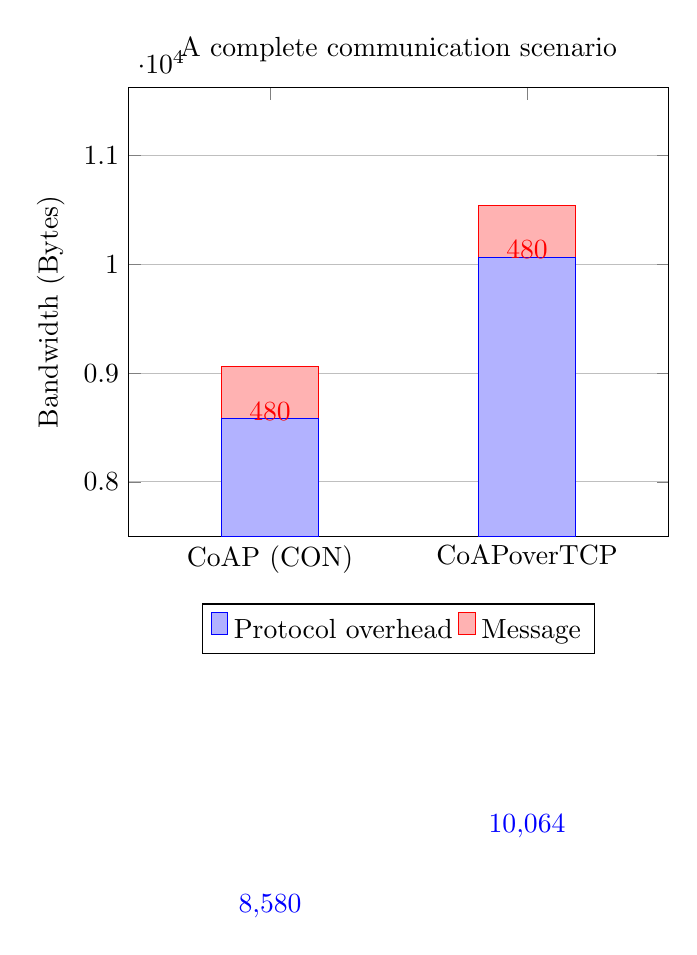
\begin{tikzpicture}
\begin{axis}[
title={A complete communication scenario},
ybar stacked,
%ymax=50,
ymajorgrids,
bar width=35pt,
%width=250pt,
nodes near coords, 
%nodes near coords={\pgfmathprintnumber\pgfplotspointmeta \%},
nodes near coords align={anchor=north},%Move values in bar
every node near coord/.style={
},
enlargelimits=0.55,
legend style={at={(0.5,-0.15)},
	anchor=north,legend columns=-1},
%width=0.8*\textwidth,
ylabel={Bandwidth (Bytes)},
symbolic x coords={CoAP (CON), CoAPoverTCP},
xtick=data,
%legend pos= north east,
%x tick label style={rotate=45,anchor=east},
]
%ethernet
\addplot+[ybar] plot coordinates { (CoAP (CON),8580) 
	(CoAPoverTCP,10064) };
%ethernet
\addplot+[ybar] plot coordinates { (CoAP (CON),480) 
	(CoAPoverTCP,480) };

\legend{\strut Protocol overhead, \strut Message}
\end{axis}
\end{tikzpicture}

\subsection{Packet-loss}
Use the NetEM tool fore emulating package-loss.
More lost packet = more packet to send = more energy consumption
This is the \figurename \ref{coapovertcploss}
\begin{figure}[bh]
	\centering
	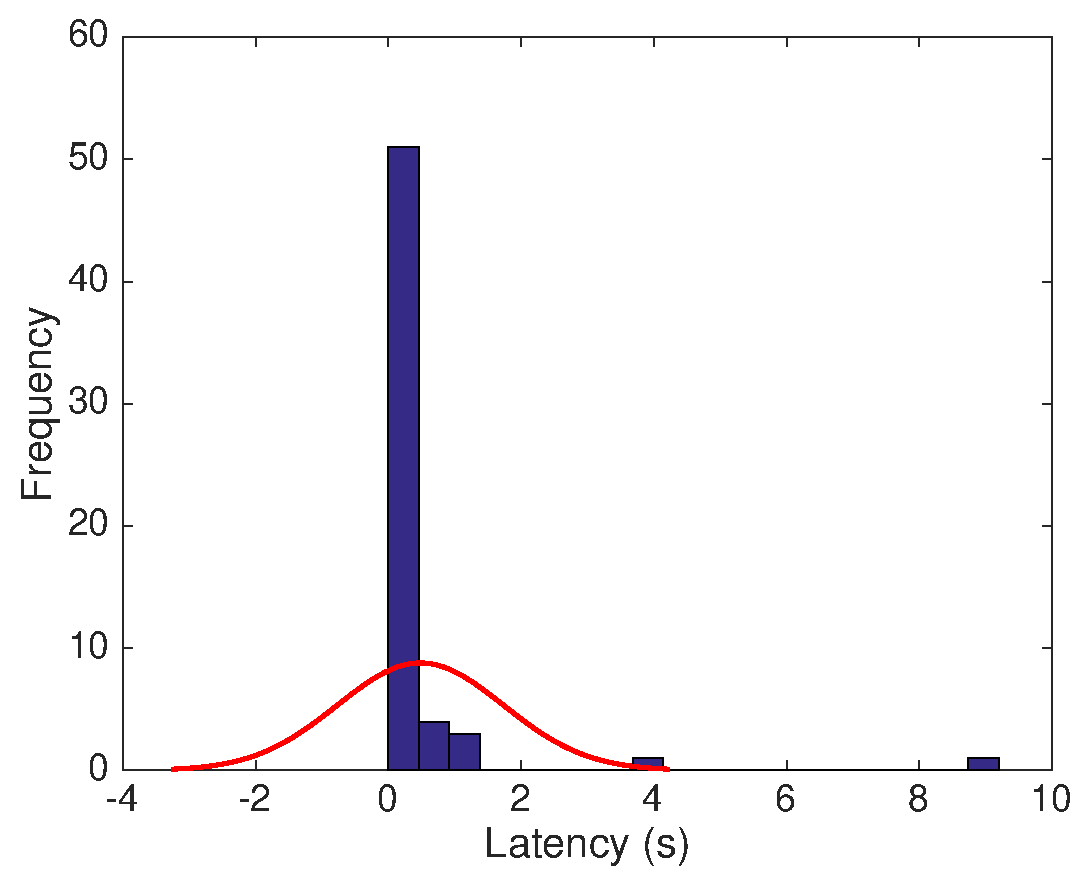
\includegraphics[width=3.5in]{gfx/coapovertcp25loss}
	\caption{Latency for CoAP over TCP with 25 \% packet loss.}
	\label{coapovertcploss}
\end{figure}

This is the \figurename \ref{coapoverudploss}
\begin{figure}[bh]
	\centering
	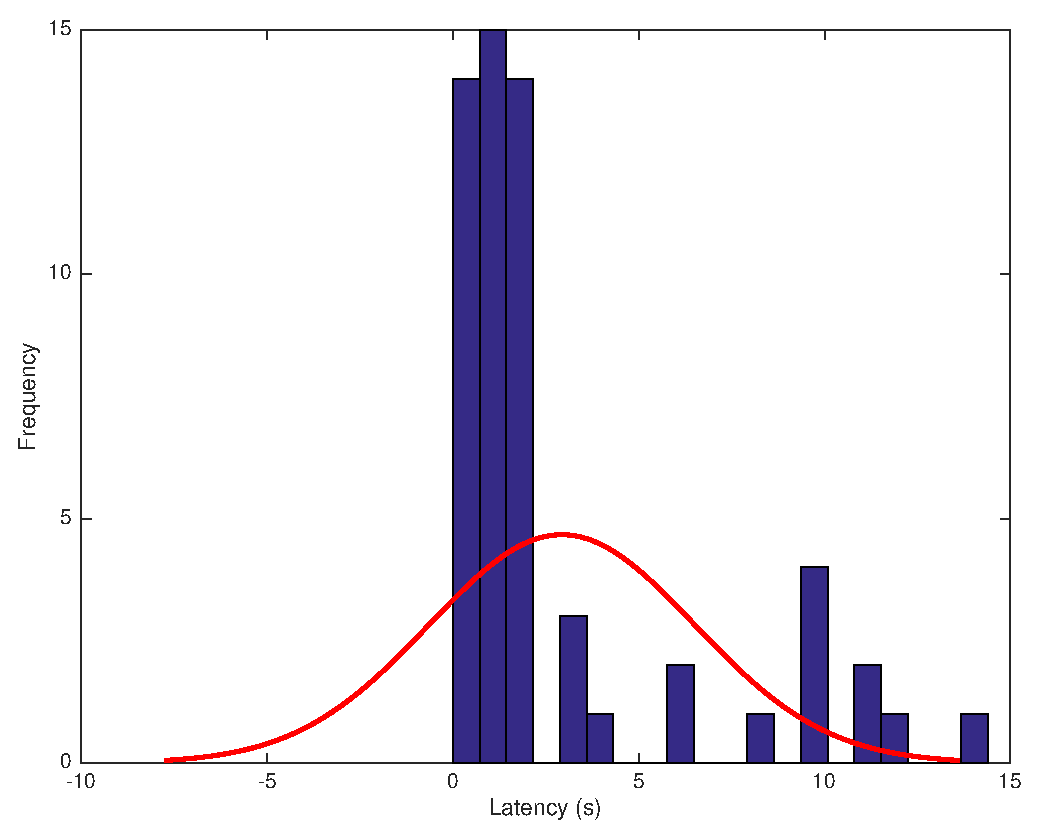
\includegraphics[width=3.5in]{gfx/coapoverudp25loss}
	\caption{Latency for CON CoAP with 25 \% packet loss.}
	\label{coapoverudploss}
\end{figure}


\subsection{Latency}
Measure RTT values %which is the time from establishing the connection to receiving the acknowledgement.
More latency = less time to sleep = more energy consumption

Spredning/fordeling/varians af delay variations 

\subsubsection{CoAP over TCP Latency}
This is the \figurename \ref{fig_sim}
\begin{figure}[bh]
\centering
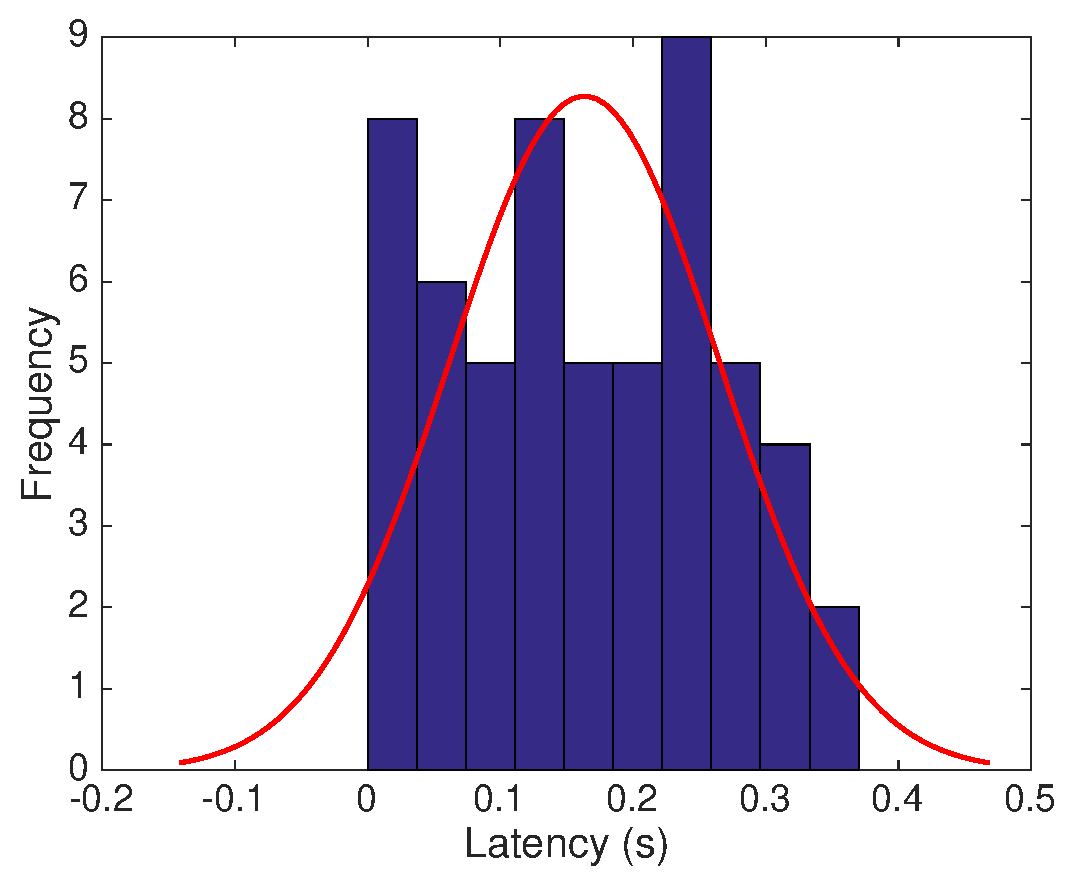
\includegraphics[width=3.5in]{gfx/coapovertcp}
\caption{Latency for CoAP over TCP without packet loss.}
\label{fig_sim}
\end{figure}

\subsubsection{Confirmable (CON) CoAP Latency}
This is the \figurename \ref{fig_sim2}
\begin{figure}[bht]
	\centering
	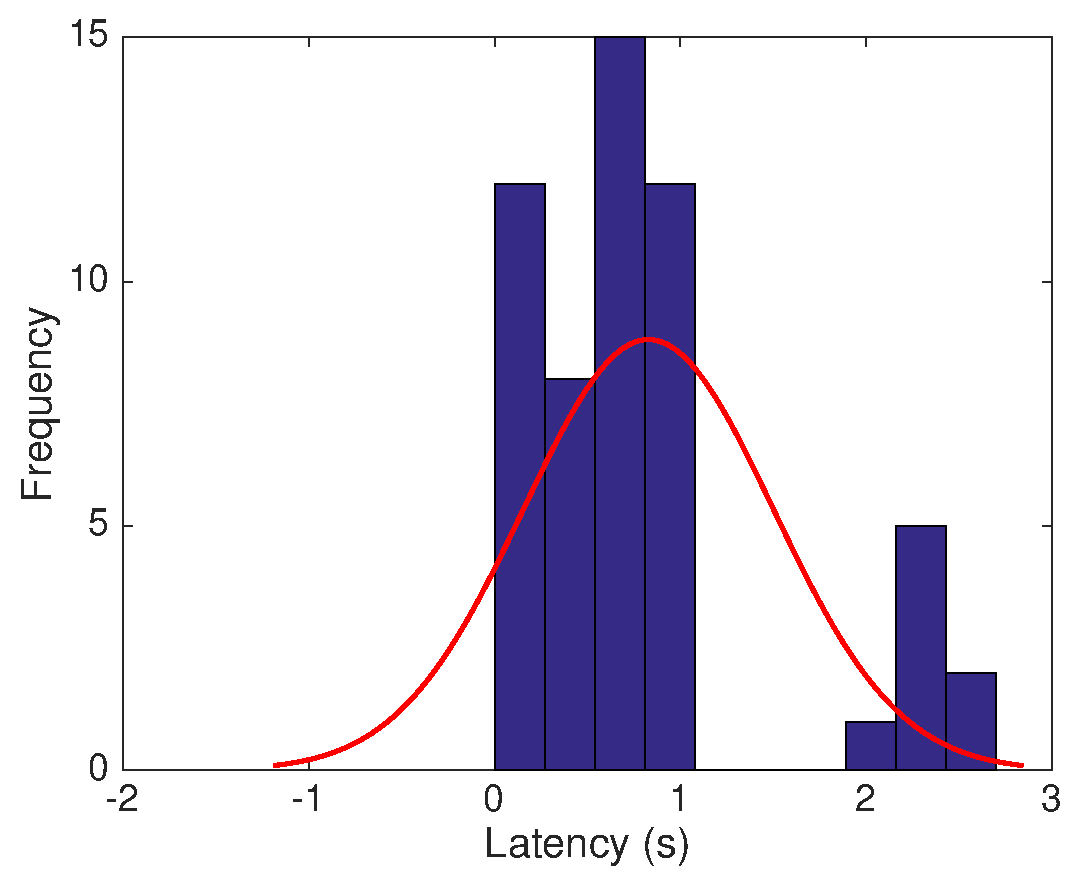
\includegraphics[width=3.5in]{gfx/coapoverudp}
	\caption{Latency for CON CoAP without packet loss..}
	\label{fig_sim2}
\end{figure}



